% --------------------------------------------------------------------------
% Formatvorlage fuer die Bacheloarbeit an der DHBW Karlsruhe, angelehnt an
% eine Vorlage von Danis Hamann auf Basis von Stefan Macke
% --------------------------------------------------------------------------
%   Angelehnt an die Vorlage von Denis Hamann auf Basis von Stefan Macke. 14.02.2011 / 12.07.2007
%   Download unter:
%   http://blog.stefan-macke.com
%   http://code.google.com/p/snmptrack/source/browse/trunk/doc/Latex/?r=550
%
%   erstellt von Julius Hacker
%   Email: info@julius-hacker.de


% Dokumentenkopf -----------------------------------------------------------
%   Diese Vorlage basiert auf "scrreprt" aus dem koma-script.
%    Die Option draft sollte beim fertigen Dokument ausgeschaltet werden.
% --------------------------------------------------------------------------
\documentclass[
  pdftex,
  fontsize=12pt,          % Schriftgroesse
  DIV10,                  % Angabe bzgl Bestimmung der Seitenabstaende
  ngerman,                % fuer Umlaute, Silbentrennung etc.
  paper=a4,               % Papierformat
  twoside=false,          % einseitiges Dokument
  titlepage,              % es wird eine Titelseite verwendet
  parskip=half,           % Abstand zwischen Absaetzen (halbe Zeile)
  headings=normal,        % Groesse der Ueberschriften verkleinern
  liststotoc,             % Verzeichnisse im Inhaltsverzeichnis auffuehren
  bibtotoc,               % Literaturverzeichnis im Inhaltsverzeichnis auffuehren
  index=totoc,            % Index im Inhaltsverzeichnis auffuehren
  captions=tableheading,  % Beschriftung von Tabellen oberhalb ausgeben
  final                   % Status des Dokuments (final/draft)
]{scrreprt}


\usepackage[utf8]{inputenc} % UTF-8 als Zeichenkodierung der Quelldateien festlegen. Wichtig wg Umlauten
\usepackage{tgheros}
\renewcommand*\familydefault{\sfdefault}
\usepackage[T1]{fontenc}
\usepackage{textcomp} % Euro-Zeichen etc.

% Informationen ------------------------------------------------------------
%   Definition von globalen Parametern, die im gesamten Dokument verwendet
%   werden knnen (z.B auf dem Deckblatt etc.).
% --------------------------------------------------------------------------
\newcommand{\titel}{Erstellen einer Android App für die Esport-Webseite readmore.de}
\newcommand{\untertitel}{Leer}
\newcommand{\art}{Studienarbeit}
\newcommand{\fachgebiet}{Angewandte Informatik}
\newcommand{\autor}{Tobias Bechtold}
\newcommand{\matrikelnr}{6463863}
\newcommand{\studienbereich}{Angewandte Informatik}
\newcommand{\kursbez}{TINF12B2}
\newcommand{\firmenname}{Fiducia IT AG}
\newcommand{\jahr}{2015}
\newcommand{\abgabedatum}{30. Mai 2015}

% Eigene Befehle
\newcommand{\todo}[1]{\textbf{\textsc{\textcolor{red}{(TODO: #1)}}}}

% Autorennamen in small caps
\newcommand{\AutorZ}[1]{\textsc{#1}}
\newcommand{\Autor}[1]{\AutorZ{\citeauthor{#1}}}

% Befehle zur semantischen Auszeichnung von Text
\newcommand{\NeuerBegriff}[1]{\textbf{#1}}
\newcommand{\Fachbegriff}[1]{\textit{#1}}
\newcommand{\Prozess}[1]{\textit{#1}}
\newcommand{\Webservice}[1]{\textit{#1}}
\newcommand{\Eingabe}[1]{\texttt{#1}}
\newcommand{\Code}[1]{\texttt{#1}}
\newcommand{\Datei}[1]{\texttt{#1}}
\newcommand{\Datentyp}[1]{\textsf{#1}}
\newcommand{\XMLElement}[1]{\textsf{#1}}

% Abkuerzungen
\newcommand{\vgl}{Vgl.\ }
\newcommand{\ua}{\mbox{u.\,a.\ }}
\newcommand{\zB}{\mbox{z.\,B.\ }}
\newcommand{\bs}{$\backslash$}

% Anpassung des Seitenlayouts ----------------------------------------------
%   siehe Seitenstil.tex
% --------------------------------------------------------------------------
\usepackage[
  automark,     % Kapitelangaben in Kopfzeile automatisch erstellen
  headsepline,  % Trennlinie unter Kopfzeile
  ilines        % Trennlinie linksbndig ausrichten
]{scrpage2}


% Anpassung an Landessprache -----------------------------------------------
%   Verwendet globale Option german siehe \documentclass
% --------------------------------------------------------------------------
\usepackage{babel}

\usepackage[printonlyused]{acronym}

% Grafiken -----------------------------------------------------------------
%     Einbinden von Grafiken [draft oder final]
%     Option [draft] bindet Bilder nicht ein - auch globale Option
% --------------------------------------------------------------------------
\usepackage[dvips,final]{graphicx}
\graphicspath{{Bilder/}} % Dort liegen die Bilder des Dokuments


% Fuer Index-Ausgabe; \printindex -------------------------------------------
\usepackage{makeidx}

% Einfache Definition der Zeilenabstaende und Seitenrnder etc. -------------
\usepackage{setspace}
\usepackage{geometry}


\usepackage{xcolor} 
\definecolor{hellgelb}{rgb}{1,1,0.9}
\definecolor{colKeys}{rgb}{0,0,1}
\definecolor{colIdentifier}{rgb}{0,0,0}
\definecolor{colComments}{rgb}{1,0,0}
\definecolor{colString}{rgb}{0,0.5,0}
\definecolor{pblue}{rgb}{0.13,0.13,1}
\definecolor{pgreen}{rgb}{0,0.5,0}
\definecolor{pred}{rgb}{0.9,0,0}
\definecolor{pgrey}{rgb}{0.46,0.45,0.48}

% Lange URLs umbrechen etc. -------------------------------------------------
\usepackage{url}

\usepackage{footnote} % Ermoeglicht Fussnoten in gleitenden Umgebungen
\makesavenoteenv[figure*]{figure}

\pdfcompresslevel=1
%\pdfimageresolution=1200
%\pdfpkresolution=1200

% Zum fortlaufenden Durchnummerieren der Fussnoten ---------------------------
\usepackage{chngcntr}

\usepackage{caption}

\usepackage{tocloft}

\newcommand{\myappendix}[1]{%
  \refstepcounter{appendix}%
  \section*{\theappendix\space #1}%
  \addcontentsline{app}{appendix}{\protect\numberline{\theappendix}#1}%
  \par
}

\newcommand{\subappendix}[1]{%
  \refstepcounter{subappendix}%
  \subsection*{\thesubappendix\space #1}%
  \addcontentsline{app}{subappendix}{\protect\numberline{\thesubappendix}#1}%
}

% Formatierung von Listen ndern
\usepackage{paralist}
% Standardeinstellungen:
% \setdefaultleftmargin{2.5em}{2.2em}{1.87em}{1.7em}{1em}{1em}

%Zeilenabstand
\renewcommand{\baselinestretch}{1.5}\normalsize

%Schriftart
\renewcommand{\familydefault}{\sfdefault}


\usepackage[see, commabeforerest, authorformat=year]{jurabib}
\renewcommand*{\bibbtasep}{; } % bta = between two authors sep
\renewcommand*{\bibbfsasep}{; } % bfsa = between first and second author sep
\renewcommand*{\bibbstasep}{; }% bsta = between second and third author sep
\renewcommand*{\bibatsep}{, }
\DeclareRobustCommand{\jbaensep}{,}

% PDF-Optionen --------------------------------------------------------------
\usepackage[
bookmarks,
bookmarksopen=true,
pdftitle={\titel},
pdfauthor={\autor},
pdfcreator={\autor},
pdfsubject={\titel},
pdfkeywords={\titel},
pdfmenubar=true,
colorlinks=true,
linkcolor=black, % einfache interne Verknpfungen
anchorcolor=black,% Ankertext
citecolor=black, % Verweise auf Literaturverzeichniseintrge im Text
filecolor=black, % Verknpfungen, die lokale Dateien ffnen
menucolor=black, % Acrobat-Menpunkte
urlcolor=black,
plainpages=false,% zur korrekten Erstellung der Bookmarks
pdfpagelabels,% zur korrekten Erstellung der Bookmarks
hypertexnames=false,% zur korrekten Erstellung der Bookmarks
linktocpage % Seitenzahlen anstatt Text im Inhaltsverzeichnis verlinken
]{hyperref}

\usepackage[T1]{fontenc}
\usepackage{inconsolata}

% Algorithmen-Formattierung
%\usepackage{algorithm}
\usepackage[final]{listings}
\lstset{language=Java,
  showspaces=false,
  showtabs=false,
  breaklines=true,
  showstringspaces=false,
  breakatwhitespace=true,
  commentstyle=\color{pgreen},
  keywordstyle=\color{pblue},
  stringstyle=\color{pred},
  basicstyle=\ttfamily\linespread{0.2},
  moredelim=[il][\textcolor{pgrey}]{$$},
  moredelim=[is][\textcolor{pgrey}]{\%\%}{\%\%}
}


\makeindex

% Zeilenabstand ------------------------------------------------------------
%\onehalfspacing
\setstretch{1,5}

% Seitenraender -------------------------------------------------------------
\geometry{paper=a4paper,left=30mm,right=25mm,top=40mm, bottom=37mm, footskip=10mm}


% Kopf- und Fusszeilen ------------------------------------------------------
\pagestyle{scrheadings}

% Kopf- und Fusszeile auch auf Kapitelanfangsseiten -------------------------
\renewcommand*{\chapterpagestyle}{scrheadings}

% Schriftform der Kopfzeile -------------------------------------------------
\renewcommand{\headfont}{\normalfont}

% Kopfzeile -----------------------------------------------------------------
\ihead{\headmark} %\small{\untertitel}
\chead{\hspace{1mm}}
\ohead{Seite \thepage}
\setlength{\headheight}{21mm} % Hhe der Kopfzeile
\setheadsepline[text]{0.4pt} % Trennlinie unter Kopfzeile

% Fusszeile -----------------------------------------------------------------
%\ifoot{\copyright\ \autor}
\cfoot{\hspace{1mm}}
\ofoot{\hspace{1mm}}


%Abbildungen
%Figures anpassung
\makeatletter
\@removefromreset{figure}{chapter}
\renewcommand*\thefigure{\@arabic\c@figure}
\makeatother


% erzeugt ein wenig mehr Platz hinter einem Punkt --------------------------
\frenchspacing 

% Schusterjungen und Hurenkinder vermeiden
\clubpenalty = 10000
\widowpenalty = 10000 
\displaywidowpenalty = 10000

% Fussnoten fortlaufend durchnummerieren ------------------------------------
\counterwithout{footnote}{chapter}

\hyphenation{SAP-An-wen-dungen}
\hyphenation{SAP-An-wen-dung}
\hyphenation{An-wen-dungen}
\hyphenation{An-wen-dung}
\hyphenation{MVC-ähn-lich-em}



% Beginn des eigentlichen Dokuments
\begin{document}

% auch subsubsection nummerieren
\setcounter{secnumdepth}{3}
\setcounter{tocdepth}{2}

% keine Kopf-/Fusszeilen bei Deckblatt und Abstract
\ofoot{}
\ohead{}

\begingroup 
\setlength{\leftmargin}{-20mm}
\setlength{\rightmargin}{10mm}
\setlength{\topmargin}{-20mm}
\setlength{\footskip}{-10mm}
\thispagestyle{plain}
\begin{titlepage}

\begin{center}

\includegraphics[scale=1.4]{Bilder/dhbw_large.jpg}

\large{\textbf{Studiengang Angewandte Informatik}}\\[6ex]

\huge{\textsc{\textbf{\titel}}}\\[4.5ex]

\large{\textbf{\art}}\\[0ex]
\large{im Rahmen der Pr\"ufung zum Bachelor of Science (B. Sc.)}\\[25mm]

\normalsize
\begin{tabbing}
\hspace*{3cm}\=\hspace*{6cm}\=\hspace{6cm}\=\kill
\>Verfasser \>\autor\\
\>Kurs \>\kursbez\\
\>Ausbildungsbetrieb \>\firmenname\\
\>Abgabedatum \>\abgabedatum\\
\end{tabbing}
\end{center}
\end{titlepage}

\endgroup

\ohead{Seite \thepage}
%\ofoot{\pagemark}

% Seitennummerierung -------------------------------------------------------
%    Vor dem Hauptteil werden die Seiten in grossen roemischen Ziffern 
%    nummeriert...
% --------------------------------------------------------------------------
\pagenumbering{Roman}

%Ueberschrifthack
\parindent 0pt
\renewcommand*{\chapterheadstartvskip}{\vspace*{0pt}}


\addchap{Sperrvermerk}

Die nachfolgende Arbeit enthält vertrauliche Daten und Informationen der Fiducia IT AG. Veröffentlichungen oder Vervielfältigungen -- auch nur auszugsweise -- sind ohne ausdrückliche schriftliche Genehmigung des Unternehmens nicht gestattet. Die Arbeit ist nur den Korrektoren sowie den Mitgliedern des Prüfungsausschusses zugänglich zu machen.
 % Sperrvermerk - wichtig bei internen Informationen aus der Firma!
\addchap{Eidesstattliche Erkl\"arung}

Ich erkl\"are hiermit eidesstattlich, dass ich die vorliegende Arbeit selbstst\"andig und ohne Benutzung anderer als der angegebenen Hilfsmittel angefertigt habe. Aus den benutzten Quellen direkt oder indirekt \"ubernommene Gedanken habe ich als solche kenntlich gemacht.

Diese Arbeit wurde bisher in gleicher oder \"ahnlicher Form oder auszugsweise noch keiner anderen Pr\"ufungsbehörde vorgelegt und auch nicht ver\"offentlicht.

\begin{tabbing}
\hspace*{10.5cm}\=\hspace*{6cm}\=\kill
Karlsruhe, den \today \>\rule[-0.2cm]{5cm}{0.5pt}\\
\>\autor\\
\end{tabbing}
   % Selbstaendigkeitserklaerung 


%Inhaltsverzeichnis einbinden
\tableofcontents 
\addtocontents{toc}{\protect\thispagestyle{scrheadings}}



%Hack fuer listoffigures
\begingroup
\renewcommand*{\addvspace}[1]{}
\newpage
\renewcommand{\cftfigpresnum}{Abb. }
\renewcommand{\cfttabpresnum}{Tab. }
\setlength{\cftfignumwidth}{2cm}
\setlength{\cfttabnumwidth}{2cm}
\addcontentsline{toc}{chapter}{\listfigurename}
\listoffigures
\addtocontents{lof}{\protect\thispagestyle{scrheadings}}
\newpage
\endgroup

% Abbildungsverzeichnis
\begingroup
\ihead{Abk\"urzungsverzeichnis}
\chapter*{Abkürzungsverzeichnis}

\addcontentsline{toc}{chapter}{\protect{Abkürzungsverzeichnis}}

\begin{acronym}[RDBMSRDBMS]
\setlength{\itemsep}{-\parsep}
\acro{ANSI/SPARC}{American National Standards Institute, Standards Planning And Requirements Committee}
\acro{CLP}{Command Line Processor}
\acro{CPU}{Central Processing Unit}
\acro{CRUD}{Create, Read, Update, Delete}
\acro{DB2 LUW}{DB2 Linux, Unix, Windows}
\acro{DBMS}{Da\-ten\-bank\-ma\-nage\-mentsys\-tem}
\acro{DCL}{Data Control Language}
\acro{DDL}{Data Definition Language}
\acro{DML}{Data Manipulation Language}
\acro{EC}{Electronic Cash}
\acro{FLOPS}{Floating Point Operations Per Second}
\acro{IDA}{agree\textregistered~Analysen Individuelle Auswertungen}
\acro{MIPS}{Million Instructions Per Second}
\acro{OLAP}{Online Analytical Processing}
\acro{OLTP}{Online Transaction Processing}
\acro{SLA}{Service Level Agreement}
\acro{SQL}{Structured Query Language}
\acro{TPC}{Transaction Processing Performance Council}
\acro{TPS}{Transactions per second}
\acro{UOW}{Unit of Work}
\end{acronym}

\endgroup

%\begingroup
%\addcontentsline{toc}{chapter}{\listtablename}
%\listoftables          % Tabellenverzeichnis
%\endgroup
%\renewcommand{\lstlistlistingname}{Verzeichnis der Listings}
%\lstlistoflistings      % Listings-Verzeichnis

% ...danach in normalen arabischen Ziffern ---------------------------------
\clearpage
\clearpage
\pagenumbering{arabic}


% Inhalt
\chapter{Einleitung}
\label{cha:Einleitung}

\section{Einleitung}
Seit dem Jahr 2005 stellt die Esport-Webseite readmore.de Informationen über
alle aktuellen Esport-Titel, laufende Turniere und News über die Esport-Szene
bereit. Ein weiterer großer Teil der Seite stellt das sehr hoch frequentierte
Forum als Diskussionsplattform rund um den Esport dar. Esport bezeichnet dabei
den sportlichen Wettkampf zwischen Menschen mithilfe von Computerspielen. Diese
Wettkämpfe werden meist im Mehrspielermodus der Spiele entweder allein oder in
einer Mannschaft ausgetragen.\footcite{TEST1234} Die aktuell am häufigsten
gespielten und mit den höchsten Preisgeldern dotierten Spiele sind unter anderem \Fachbegriff{Dota 2},
\Fachbegriff{Starcraft 2} und \Fachbegriff{Counter-Strike: Global Offensive}.
Mit Preisgeldern bis zu einer Million US-Dollar pro Turnier zieht alleine der
Esport-Titel \Fachbegriff{Dota 2} über 10 Millionen Spieler weltweit
an.\footnote{Quelle:
http://steamcharts.com/}
Das Forum der Esport-Webseite readmore.de stellt dabei eine der größten
Diskussionsplattformen im deutschsprachigen Raum dar. \\
Allerdings gibt es über 10 Jahre nach der Gründung der Seite noch keine
Möglichkeit, die Seite auf mobilen Endgeräten wie Smartphones oder Tablets in
einer dafür optimierten Ansicht zu betrachten. Die einzige verfügbare Ansicht
ist die Desktopansicht der Seite. Daher sollen in dieser Studienarbeit die
technischen Möglichkeiten untersucht werden, wie diese Seite auch mit mobilen
Endgeräten einfacher betrachtet werden kann. Dies soll mithilfe einer Android
App möglich werden.
\section{Aufgabe und Problemstellung}
Um die readmore.de Webseite auch auf mobilen Endgeräten darzustellen soll eine
Android App entwickelt werden. Diese soll die wichtigste Funktion der Seite, das
Forum, mit nativen Android Komponenten anzeigen. Zusätzlich soll sich der
Benutzer mit seinem readmore.de-Account einloggen und somit auch aktiv im Forum
posten können. Da readmore.de keine API bereitstellt besteht ein wichtiger Teil
der Aufgabe im Auslesen der auf der Webseite angezeigten Daten, wie Foren, Threads und Beiträge. Diese
Aufgabe kann unter Umständen mit einer eigenen Serverkomponente gelöst werden.
Die Kommunikation der App findet dann nicht mehr direkt mit readmore.de statt,
sondern mit einem selbst entwickelten Server der die angeforderte Seite in einem
schnell auslesbaren Format zurückliefert. 
\section{Motivation und Herausforderung}

\chapter{Konzeption und theoretische Grundlagen}
\label{cha:theoGrundlagen}

\section{Android App-Entwicklung}
Android ist ein auf dem Linux Kernel basierendes mobiles Betriebssystem. Zur
Zeit wird Android von Google entwickelt und zielt auf Geräte ab, die über einen
Touchscreen bedient werden. Dazu zählen Smartphones, Tablets und neuerdings auch
Smartwatches. Wie üblich bei auf Linux basierenden Betriebssystemen, ist auch
der Android Quellcode unter der \Fachbegriff{open source} Lizenz frei verfügbar.
Der Funktionsumfang des Betriebssystems lässt sich durch Apps beliebig
erweitern. Diese Apps können vom Benutzer aus dem \Fachbegriff{Google Play
Store} bezogen werden. Der \Fachbegriff{Play Store} stellt die zentrale App
dar, in der alle Apps katalogisiert sind die mithilfe des \Fachbegriff{Android
SDK} entwickelt wurden. \\
Das \Fachbegriff{Android Software Development Kit} bietet neben verschiedenen
Entwicklungswerkzeugen auch eine eigene Entwicklungsumgebung an. Zu den
verschiedenen Entwicklungswerkzeugen zählen unter anderem ein Debugger, die
Android Bibliotheken und ein Emulator der verschiedene mobile Endgeräte zu
Testzwecken emulieren kann. Dieser Emulator ermöglicht das Testen von Android
Applikationen falls kein physisches Gerät zur Verfügung steht. Die Kommunikation
mit physischen Geräten, beispielsweise um das Debugging von Apps auf dem Gerät
zu ermöglichen, findet über die Android Debug Bridge (ADB) statt. \\
Android Applikationen werden in \Fachbegriff{Java} entwickelt. Java ist eine 
objektorientierte Programmiersprache.
Java Quellcode wird vom Java Compiler in Bytecode umgewandelt, welcher
nicht wie bei anderen Programmiersprachen üblich direkt durch Hardware ausgeführt
wird, sondern auf einer virtuellen Maschine (der Java Virtual Machine) läuft.
Dies sorgt für die oft beworbene Plattformunabhängigkeit von Java. Ob Windows,
Mac, Linux oder mobile Betriebssysteme wie z.B Android, das Java Prinzip „Write
once run anywhere“ bringt Java auf mehr als 50 Mio. PCs und Milliarden von verschiedensten
Geräten weltweit.\footcite{sierra2006} \\
Die Entwicklung mit dem Android SDK unterscheidet sich nur an manchen Stellen
von klassischer Java Entwicklung. Viele native Java Bibliotheken können auch in
der Android Entwicklung eingesetzt werden. Die Entwicklung von Oberflächen
unterschiedet sich jedoch etwas von der klassischen Oberflächenentwicklung mit
\Fachbegriff{Java Swing}. Android Oberflächen werden in sogenannte
\Fachbegriff{Activities} unterteilt. Üblicherweise ist jeder
\Fachbegriff{Activity} eine bestimmte Oberfläche zugeordnet. Mithilfe der
verschiedenen \Fachbegriff{Activities} wird in erster Linie die Navigation
innerhalb der App gesteuert. Die \Fachbegriff{Activities} reagieren auf Gesten
und Tastendrücke des Benutzers. Sollte also ein Benutzer beispielsweise den
\Fachbegriff{Zurück} Button auf seinem Gerät drücken, so wechselt die App auf
die zuvor angezeigte \Fachbegriff{Activity}. \Fachbegriff{Activities} können
sich auch gegenseitig aufrufen und stellen somit
den Navigationsfluss innerhalb der App sicher.\footcite{künneth2012android}

\section{Eingesetzte Technologien}
\subsection{Jsoup}
Um die Informationen im readmore.de Forum, also verschiedene Foren und Beiträge,
auszulesen, wird die Java Bibliothek \Fachbegriff{jsoup} auf der
Serverseite eingesetzt.
\Fachbegriff{jsoup} ist eine Bibliothek mit der es möglich ist, HTML Dateien zu
parsen und die enthaltenen Informationen zu extrahieren. \Fachbegriff{jsoup}
bietet hierzu die Möglichkeit die Baumstruktur des eingelesenen HTML Dokuments
zu durchlaufen und beispielsweise nach bestimmten Attributen zu filtern. Dazu
bietet die Bibliothek mit der sogenannten \Fachbegriff{Selektor Syntax} eine
Manipulationssprache um bestimmte Elemente im \Fachbegriff{DOM} des HTML
Dokument zu selektieren. Ein \Fachbegriff{DOM} ist in diesem Kontext die 
Baumstruktur in der das HTML Dokument strukturiert ist. \\
\subsection{Restlet}
Damit der Server auch von außen über HTTP Requests erreichbar ist, wurde das
Framework \Fachbegriff{Restlet} eingesetzt um eine \Fachbegriff{RESTful}
Serverkomponente bereit zu stellen. Das Programmierparadigma Representational
State Transfer (kurz: REST) beschreibt eine Serverkomponente die lediglich
unveränderte Seiteninhalte zum Abruf bereitstellt. Die Kommunikation mit dieser
Serverkomponente erfolgt über verschiedene HTTP-Methoden. Um beispielsweise
Daten vom Server abzurufen wird die Methode \Fachbegriff{GET} verwendet. Der Zustand am Server
wird dadurch nicht verändert. Restlet bringt eine fertige Serverkomponente mit
die nur noch an einem Port registriert werden muss. Über einen
\Fachbegriff{Router} werden dann Adressen verteilt die auf einzelne
\Fachbegriff{Restlets} verweisen. Wird also die URL eines \Fachbegriff{Restlets}
aufgerufen, reagiert das \Fachbegriff{Restlet} mit seiner Methode
\Code{handle()} auf die Anfrage. Dort werden dann die eventuellen Parameter des
GET-Requests ausgelesen, die Anfrage wird verarbeitet und anschließend wird die
angeforderte Ressource zurückgegeben. Nachfolgend ein Beispiel einer einfachen
\Fachbegriff{Restlet}-Serverkomponente mit einem Restlet.
\begin{lstlisting}[caption=Die Serverkomponente, label=komponente]
public class ReadmoreServer extends Application {
	private static ThreadsRestlet threadsRestlet;
	private static ForumRestlet forumRestlet;
	private static BeitragRestlet beitragRestlet;
	static {
		threadsRestlet = new ThreadsRestlet();
		forumRestlet = new ForumRestlet();
		beitragRestlet = new BeitragRestlet();
	}
	public static void main(String[] args) throws Exception {
		Component component = new Component();
		component.getServers().add(Protocol.HTTP, 8182);
		ReadmoreServer server = new ReadmoreServer();
		component.getDefaultHost().attach("", server);
		component.start();
	}
	public Restlet createInboundRoot() {
	    Router router = new Router(getContext());
	    router.attach("/threads", threadsRestlet);
	    router.attach("/forum", forumRestlet);
	    router.attach("/beitrag", beitragRestlet);
	    return router;
	  }
}
\end{lstlisting}
Wie in \ref{komponente} zu sehen, hört die Serverkomponente auf einen bestimmten
Port. In der Methode \Code{createInboundRoot()} wird mithilfe des \Code{Router}
die Adressen auf die die einzelnen Restlets reagieren festgelegt. Nachfolgend
ein einfaches \Fachbegriff{Restlet}
\begin{lstlisting}[caption=Ein einfaches Restlet, label=restlet]
public class ForumRestlet extends Restlet {
	@Override
    public void handle(Request request, Response response) {
		List<Forum> forum = getForum();
        String message = null;
        Gson gson = new Gson();
        message = gson.toJson(forum);
        response.setEntity(message, MediaType.TEXT_PLAIN);
    }
	private List<Forum> getForum() {
		ForenParser tp = new ForenParser();
		return tp.getForen();
	}
}
\end{lstlisting}
Die Methode \Code{handle(Request request, Response response)} legt beim Aufruf
des Restlets die \Fachbegriff{Response}, also die Antwort des Servers fest die
beim Aufruf zurückgegeben wird.
\subsection{Gson}
Das von Google entwickelte Framework \Fachbegriff{Gson} bietet die Möglichkeit
Java-Objekte vollautomatisch in das \Fachbegriff{JSON}-Format zu übertragen und
umgekeht \Fachbegriff{JSON}-Objekte in existierende Java-Objekte zu
transferieren.\footnote{https://sites.google.com/site/gson/gson-user-guide} 
\Fachbegriff{Gson} wird auf der Serverkomponente zur Erstellung der Antwort auf
GET Anfragen verwendet. 
\section{Konzeption des Servers}
Die Serverkomponente der Readmore App dient in erster Linie dem Auslesen der
sichtbaren Informationen im Forum von readmore. Dazu gehören die verschiedenen
Foren die in verschiedene Kategorien unterteilt sind, die Threads, also die
Einträge in jedem gewählten Forum und die einzelnen Beiträge auf jeder Seite
eines gewünschten Threads. 
\begin{figure*}[!htbp]
\centering
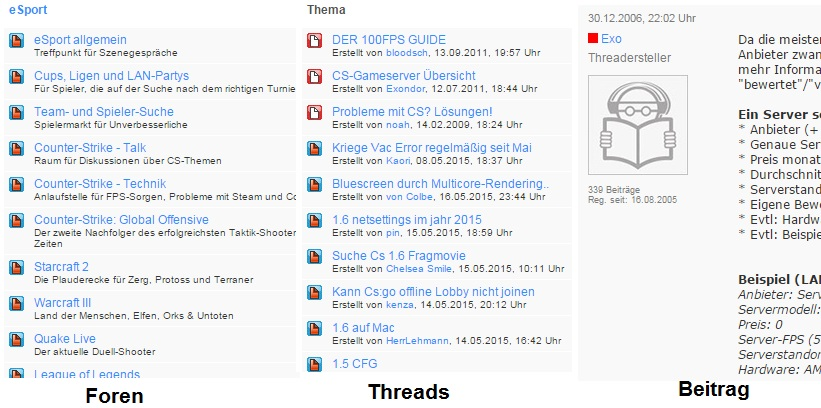
\includegraphics[width=\textwidth]{Bilder/ftb.jpg}
\caption[Foren, Threads und Beiträge auf Readmore]{Foren, Threads und Beiträge auf Readmore\protect\footnote{eigene Darstellung.} }
\label{dminfo}
\end{figure*}
Die App soll also nicht direkt mit readmore.de kommunizieren sondern bekommt
alle zur Anzeige des Forums relevanten Informationen in einem schnell zu
verarbeitenden Format. Dieses Vorgehen legt das aufwendige traversieren durch
den HTML-Code von readmore.de auf den Server um, und spart somit wertvolle
Ressourcen des Mobilgeräts ein.
\section{Anforderungen an die Oberfläche}
Use Cases, Mockups der Oberfläche usw.
\chapter{Implementierung}

\section{Implementierung des Servers}
\subsection{Parsen der Informationen mit Jsoup}
Um die nötigen Informationen über Foren, Threads und Beiträge für die App
bereitzustellen, müssen diese aus dem bestehenden HTML von readmore.de
ausgelesen werden. Dazu wird das im vorherigen Kapitel schon beschriebene
Framework \Fachbegriff{jsoup} eingesetzt. Um die Informationen auszulesen,
wurden für Foren, Threads und Beiträge jeweils ein eigener Parser implementiert
wie im nachfolgenden UML-Diagramm zu sehen ist.
\begin{figure*}[!htbp]
\centering
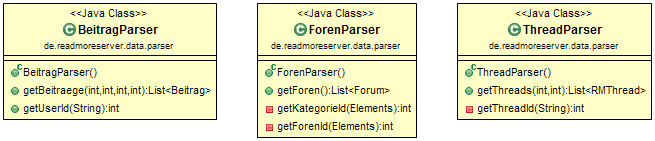
\includegraphics[width=\textwidth]{Bilder/Parser.png}
\caption[Parser für die verschiedenen Forenbereiche]{Parser für die verschiedenen Forenbereiche
 \protect\footnote{eigene Darstellung.} }
\label{dminfo}
\end{figure*}
Jeder der Parser liefert eine Liste vom Typ des jeweiligen geparsten Objekts
zurück, also entweder \Code{Forum}, \Code{RMThread} oder \Code{Beitrag}. Diese
Objekte werden zur internen Datenhaltung verwendet und während des Parsens des
HTML erstellt und mit Daten befüllt. Zusätzlich zu Foren, Threads und Beiträgen,
werden auch die Benutzer in einem eigenen Objekt abgebildet. Dort werden
notwendige Informationen zur späteren Darstellung in der App abgebildet, wie z.B
der Benutzername und der Link zum Avatar des Benutzers. Das Enum \Code{RMStatus}
bildet die Sichtbarkeit des Online Status eines Benutzers ab. Im nachfolgenden
UML-Diagramm wird der Aufbau der einzelnen Objekte dargestellt.
\begin{figure*}[!htbp]
\centering
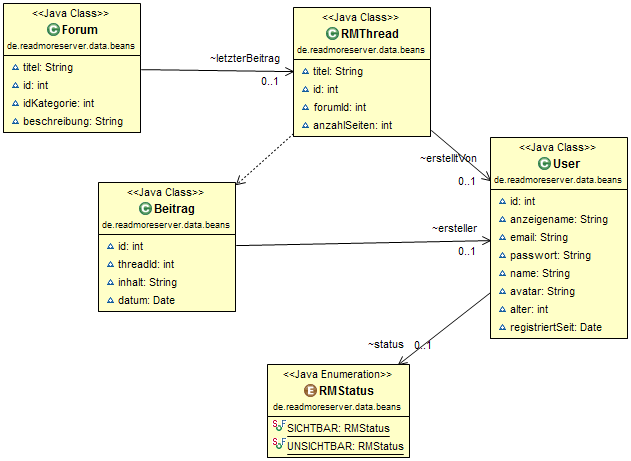
\includegraphics[width=\textwidth]{Bilder/beans.png}
\caption[Objekte für die interne Datenhaltung]{Objekte für die interne Datenhaltung \protect\footnote{eigene Darstellung.} }
\label{dminfo}
\end{figure*}
Das Parsen der HTML-Struktur findet wie schon erwähnt mit \Fachbegriff{jsoup}
statt. Das Framework bietet hierfür viele Möglichkeiten um HTML Elemente anhand
ihrer Klassen, Tags oder anderen Merkmale auszuwählen. Um eine Webseite mit
\Fachbegriff{jsoup} auszulesen, wird über die Methode \Code{connect(URL url)}
das gesamte \Code{Document} mit allen Elementen zurückgegeben. Dieses
\Code{Document} ermöglicht die Selektion der verschiedenen Elemente über die
die bereitgestellten Methoden. Nachfolgend eine Auflistung der wichtigsten
Methoden:
\begin{itemize}
  \item \Code{getElementById(String id)}
  \item \Code{getElementsByAttribute(String key)}
  \item \Code{getElementsByAttributeValue(String key, String value)}
  \item \Code{getElementsByClass(String className)}
  \item \Code{getElementsByTag(String tagName)}
\end{itemize}
Diese Methoden geben je nach Eindeutigkeit der Selektionsparameter ein
\Code{Element} oder die Wrapperklasse \Code{Elements}, die eine Liste
implementiert, zurück. Ein einzelnes \Code{Element} wird nur bei der Methode
\Code{getElementById(String id)} zurückgegeben, da eine Id in HTML Quellcode
stets eindeutig ist. Die Wrapperklasse \Code{Elements} stellt eine Liste von
\Code{Elements} dar, und enthält alle Elemente die den Selektionskriterien
entsprechen. Die implementierten Parser für für Foren, Threads und Beiträge
iterieren über verschiedene \Code{Elements}, um beispielsweise alle Foren der
Forumsstartseite zu erhalten. Diese Iteration ist im nachfolgenden Codebeispiel
zu sehen.
\begin{lstlisting}[caption=Auslesen der Foren im Forenparser, label=forenparser]
public List<Forum> getForen() {
  Document doc = Jsoup.connect("http://www.readmore.de/forums/").get();
  Elements e = doc.getElementsByClass("forum_forums");
  for (Element element : e) {
  Elements foren = element.getElementsByTag("tr");
    for(Element forum : foren) {
      if(forum.children().size() > 4) {
   	    Elements attribute = forum.children();
	    Forum f = new Forum();
	    Elements linkTitel = attribute.get(1).getElementsByTag("a");
	    f.setTitel(linkTitel.text());
	    f.setBeschreibung(attribute.get(1)
	    .getElementsByClass("second_row").text());
	    f.setIdKategorie(getKategorieId(linkTitel));
	    f.setId(getForenId(linkTitel));
	    forenListe.add(f);
      }
    }
  }
}
\end{lstlisting}
In Listing \ref{forenparser} ist auch die Traversierung durch die Baumstruktur
des HTML-Quellcodes zu sehen. Sobald die Informationen aus den einzelnen
Foren-Elementen ausgelesen wurden, wird ein neues \Code{Forum} Objekt erstellt
und mit den ausgelesenen Daten befüllt. Die Parser für Beiträge und Threads
verhalten sich analog.
\subsection{REST Schnittstelle}
Damit die ausgelesenen Daten auch von überall aus abgerufen werden können, wurde
eine REST-Schnittstelle implementiert, die die Daten per HTTP GET im
JSON Format bereitstellt. Um diese zu realisieren, wurde das Framework
\Fachbegriff{Restlet} eingesetzt. Die Klasse \Code{ReadmoreServer} bildet die
Hauptklasse des Servers. Dort wird eine neue Serverkomponente auf Port 8182
gestartet, und das Routing der verschiedenen Anfragen vorgenommen. Es existieren
drei verschiedene Adressen auf die der Server reagiert: \Code{/forum},
\Code{/threads} und \Code{/beitrag}. Eine Anfrage auf \Code{/forum} findet ohne
Parameter statt und gibt ein Json Array mit allen Foren Objekten zurück. Die
Anfragen auf \Code{/threads} und \Code{/beitrag} müssen mit Parametern versehen
werden. Um die Liste mit allen Threads eines bestimmten Forums zu bekommen
müssen die ID des Forums und die ID der Kategorie in der das Forum sich befindet
mitgegeben werden. Die Anfrage um beispielsweise alle Threads im Hardware Forum
von readmore.de abzufragen, würde sich folgendermaßen zusammen setzen:
\Code{/threads?categoryId=91\&forenId=10}.
Um Beiträge einer Seite eines bestimmten Threads zu erhalten müssen außer der
Foren-ID und der Kategorie-ID auch die ID des Threads und die gewünschte Seite
angegeben werden.
\begin{itemize}
  \item Beispiel: 
  \Code{/beitrag?categoryId=91\&forenId=10\&threadId=138573\&seite=1}
\end{itemize}
\begin{figure*}[!htbp]
\centering
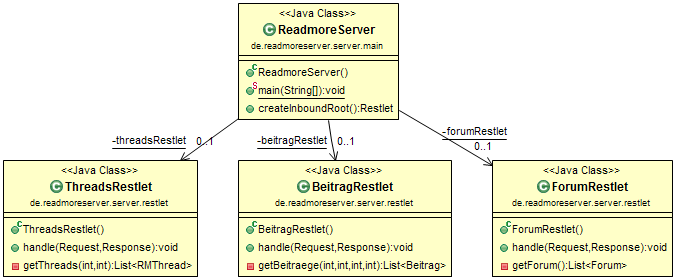
\includegraphics[width=\textwidth]{Bilder/server.png}
\caption[Architektur der REST-Schnittstelle]{Architektur der REST-Schnittstelle \protect\footnote{eigene Darstellung.} }
\label{restuml}
\end{figure*}
Die beschriebenen Anfragen werden in der Hauptklasse des Servers auf
entsprechende \Fachbegriff{Restlets} weitergeleitet, d.h. jede Anfrage 
\Code{/forum}, \Code{/threads} und \Code{/beitrag} wird auf ein eigenes Restlet
weitergeleitet. Dort wird der ankommende GET Request bearbeitet und die
entsprechende Antwort zurückgegeben. Wie im UML Diagramm \ref{restuml} zu sehen,
sind dafür die Restlets \Code{ThreadsRestlet}, \Code{BeitragRestlet} und
\Code{ForumRestlet} zuständig. 
\begin{lstlisting}[caption=Routing der Restlets, label=routing]
public Restlet createInboundRoot() {
  Router router = new Router(getContext());
  router.attach("/threads", threadsRestlet);
  router.attach("/forum", forumRestlet);
  router.attach("/beitrag", beitragRestlet);
  return router;
}
\end{lstlisting}
Wird eine Anfrage an ein Restlet weitergeleitet, wird im Restlet automatisch die
Methode \Code{handle(Request, Response)} aufgerufen. Diese bekommt den Request und eine
Response um eine Antwort zu generieren. Nachfolgend das ForumRestlet als
Beispiel wie die Rückgabe der Forenliste funktioniert.
\begin{lstlisting}[caption=Funktionsweise des ForumRestlet, label=forumrestlet]
public class ForumRestlet extends Restlet {

	@Override
    public void handle(Request request, Response response) {
		List<Forum> forum = getForum();
        String message = null;
        Gson gson = new Gson();
        message = gson.toJson(forum);
        response.setEntity(message, MediaType.TEXT_PLAIN);
    }
    
	private List<Forum> getForum() {
		ForenParser tp = new ForenParser();
		return tp.getForen();
	}
}
\end{lstlisting}
Um eine Liste aller Foren zu erhalten, wird zuerst der \Code{ForenParser}
aufgerufen. Diese Liste wird mithilfe des Frameworks \Fachbegriff{Gson} in ein
JSON Array umgewandelt. \Fachbegriff{Gson} bildet dabei alle Attribute des Java
Objekt in einem Json Objekt ab. Abschließend wird die JSON Nachricht in die HTTP
Response geschrieben. Das JSON Array enthält Forum Objekte im
nachfolgenden Format. 
\begin{lstlisting}[caption=Format der Forum Objekte,label=jsonforum] 
{"titel":"Hardware","id":10,"idKategorie":91,
"beschreibung":"Ecke fuer Technikinteressierte"}
\end{lstlisting}
\section{Implementierung der App}
Die Oberfläche der App besteht aus vier verschiedenen Acitivites. Einer Activity
für den Login, eine um die Forenübersicht darzustellen, eine um die Threads des
gewählten Forums darzustellen und eine Activity um den Thread selbst, also die
Beiträge im Thread, darzustellen. 
\begin{figure*}[!htbp]
\centering
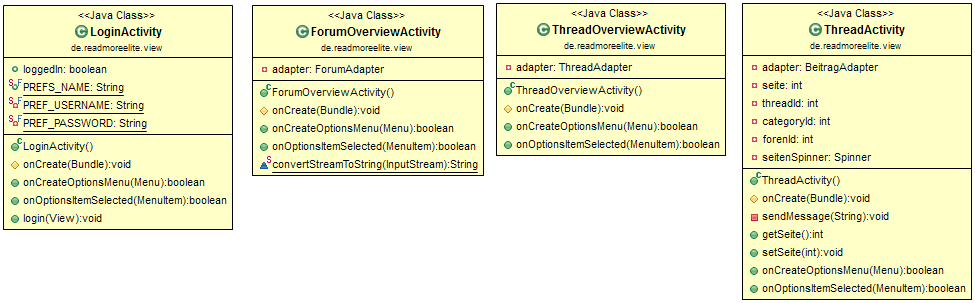
\includegraphics[width=\textwidth]{Bilder/activities.png}
\caption[Oberflächen der App]{Oberflächen der App
\protect\footnote{eigene Darstellung.} }
\label{restuml}
\end{figure*}
Die Übersichten für Foren, Threads und Beiträge werden in einer Android
\Code{ListView} dargestellt. Da Netzwerkoperationen in Android Applikationen
immer einen eigenen Thread benötigen, besitzen alle Activities einen
\Code{AsyncTask} der diese Operationen in der Methode
\Code{doInBackground()}durchführt.\\
Die \Code{LoginActivity} benötigt den \Code{AsyncTask} um den Login über
readmore.de durchzuführen. Dort wird mithilfe des \Fachbegriff{Apache HTTP
Client} ein POST mit den Logindaten durchgeführt. Der HTTP Client verwaltet
anschließend automatisch alle Cookies, die später zum erstellen von Beiträgen
benötigt werden. 
\begin{lstlisting}[caption=Durchführen des Login POST]
HttpPost post = new HttpPost(login);
post.setEntity(new UrlEncodedFormEntity(loginParams, "UTF-8"));
HttpResponse response = client.execute(post);
\end{lstlisting}
Der Quellcode zeigt wie ein POST mit dem Apache HTTP Client durchgeführt wird.
Der String \Code{login} enthält die URL der readmore.de Login Seite. \\
Die Activities zur Anzeige der Forendaten rufen in ihrem \Code{AsyncTask} die
Informationen der API ab. Diese werden in Java Objekte umgewandelt und dem
Adapter der jeweiligen \Code{ListView} weitergegeben. Jede \Code{ListView}
besitzt einen eigenen Adapter für den jeweiligen Datentyp Forum, Thread oder
Beitrag. Dieser Adapter steuert wie die Informationen in der Liste angezeigt
werden und gibt beim Klick auf ein Item in der Liste das entsprechende Java
Objekt zurück.
\begin{figure*}[!htbp]
\centering
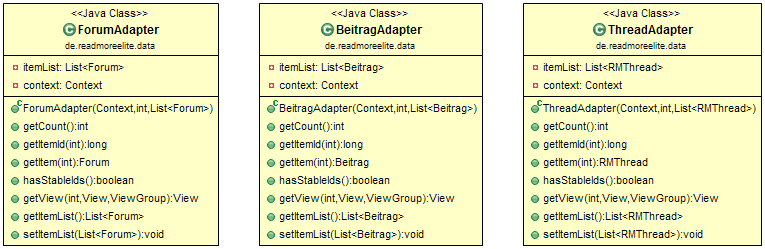
\includegraphics[width=\textwidth]{Bilder/adapter.png}
\caption[Adapter für die unterschiedlichen Datentypen]{Adapter für die unterschiedlichen Datentypen
\protect\footnote{eigene Darstellung.} }
\label{restuml}
\end{figure*}
Um dem Benutzer die Möglichkeit zu geben die Übersichten nach Wunsch zu
aktualisieren wurde eine \Fachbegriff{PullToRefresh} Logik verbaut. Das bedeutet
sobald der Benutzer am oberen Ende der List nach unten zieht, wird die Liste
aktualisiert. Dazu wird erneut der \Code{AsyncTask} ausgeführt. Diese
\Fachbegriff{PullToRefresh} Logik wird mit dem aktuellen Android SDK
mitgeliefert und nennt sich \Code{SwipeRefreshLayout}. 
\begin{figure*}[!htbp]
\centering
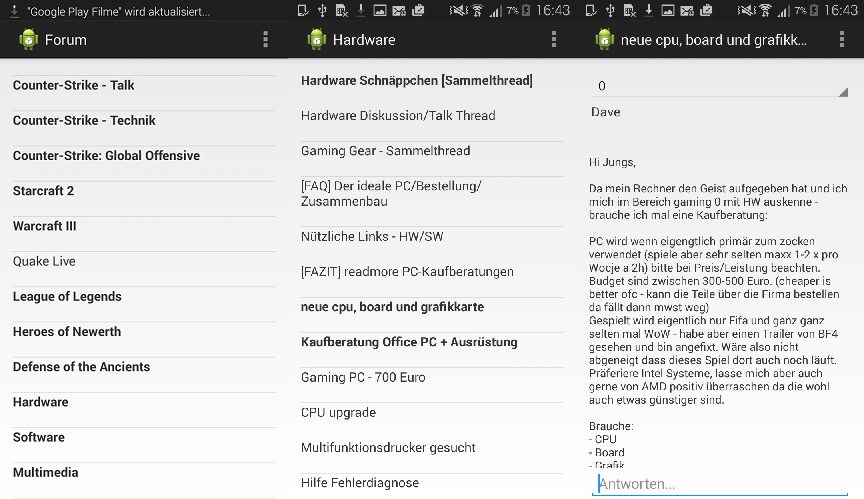
\includegraphics[width=\textwidth]{Bilder/screen_gesamt.png}
\caption[Screenshot der drei Übersichten]{Screenshot der drei Übersichten \protect\footnote{eigene Darstellung.} }
\label{restuml}
\end{figure*}

\chapter{Fazit \& Ausblick}
\label{cha:Fazit}
\section{Fazit}
In dieser Studienarbeit sollte gezeigt werden, wie eine Webseite die nicht für
Mobilgeräte optimiert ist, auf diesen Geräten angezeigt werden kann. Dazu wurden
mehrere Lösungsmöglichkeiten evaluiert. Die Entscheidung fiel auf die
Entwicklung einer eigenen API, die es ermöglicht die komplex eingebetteten Daten
im readmore.de HTML Quellcode übersichtlich und maschinell verarbeitbar
darzustellen. Desweiteren wurde auf Basis dieser API ein Prototyp einer App
entwickelt, der es ermöglicht das Forum der Webseite komfortabel auf einem
Android Smartphone zu benutzen. Der Protoyp enthält bisher zwar nur grundlegende
Funktionen, wird allerdings auch nach Fertigstellung dieser Arbeit stetig
weiterentwickelt.
\section{Ausblick}
Im Anschluss an diese Arbeit wird der Prototyp der readmore.de Android App in
einer öffentlichen Beta verprobt. Diese Beta dient in erster Linie dem Einholen
von Feedback der späteren Benutzer. Zum einen sollen potentielle Fehler
frühzeitig erkannt werden, zum Anderen können Teilnehmer der Beta ihre Ideen für
fehlende Features einbringen. Zu einem späteren Zeitpunkt ist auch die
Veröffentlichung der App im Google Play Store angedacht. \\
Durch die weite Verbreitung des Json Formats, ist die entwickelte API
plattformunabhängig. Dies lässt den Einsatz auch auf anderen
Plattformen wie iOS oder Windows Phone zu. Daher ist es in Naher Zukunft
denkbar, das Forum von readmore.de auch auf anderen mobilen Betriebssystemen
komfortabel bedienen zu können.


\pagenumbering{Roman}
\setcounter{page}{7}


% Literaturverzeichnis
\bibliography{Bibliographie}
\bibliographystyle{jurecocst}

\ihead{Quellen/Literaturverzeichnis}


\end{document}
